Il clustering, o analisi di raggruppamento, è una tecnica non supervisionata con lo scopo di aggregare i dati in \textit{cluster} o gruppi
tali che i dati all'interno di un gruppo siano più simili tra loro rispetto a quelli all'esterno\cite{liao2005clustering, zazzarro2009clustering}.

I metodi di clustering per elaborare dati statici di differenti tipologie sono cinque:

\begin{itemize}
  \item Metodi basati sul partizionamento.
  \item Metodi basati sulla gerarchia.
  \item Metodi basati sulla densità.
  \item Metdi basati su una griglia.
  \item Metodi basati sul modello.
\end{itemize}

Il clustering basato sul partizionamento si basa sull'idea di individuare \textit{k} punti e successivamente
eseguire l'assegnazione di ogni elemento del dataset a uno dei \textit{k} punti individuati nella prima fase.
In questo modo sono individuate \textit{k} partizioni, che corrispondono ad altrettanti cluster.
Questo metodo ha come vantaggio la semplicità e il ridotto numero di iperparametri,
è infatti necessario specificare a priori solo il valore di \textit{k}.
Due esempi di algoritmi~\cite{arora2016analysis} possono essere \textit{k-means} e \textit{k-medioid}:
entrambi partono dall'individuare \textit{k} punti a caso all'interno del dataset, successivamente eseguire l'assegnazione dei restanti elementi,
ricalcolare il centro del cluster in un caso, il medioide nell'altro e riperetere le operazioni fino a giungere a una convergenza ai centri dei cluster.
In figura~\cref{fig:chap-1:k-means-overview} è presentato un'esempio di esecuzione di \textit{k-means}.
I limiti di questo approccio sono l'eccessiva rigidità delle regole applicate nella generazione dei cluster e la necessità di conoscere a prescindere il numero di cluster \textit{k}.

\begin{figure}
  \centering
  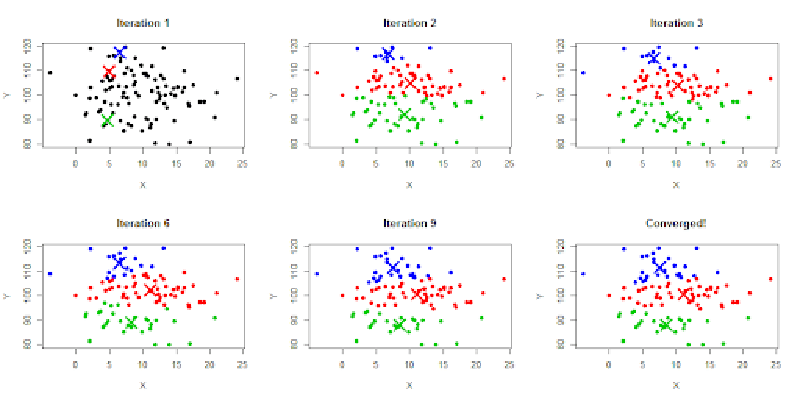
\includegraphics{/sec-1/KMeans.pdf}
  \caption{Fasi dell'algoritmo \textit{k-means},Fonte:~\url{http://www.learnbymarketing.com/methods/k-means-clustering/}}%
  \label{fig:chap-1:k-means-overview}
\end{figure}

Passando ai metodi basati sulla gerarchia, questi prevedono una divisione del dataset definendo un criterio gerarchico tra i vari elementi.
A seconda della modalità di divisione si possono individuare due categorie: se la gerarchia è definita combinando di volta in volta i singoli elementi,
allora si parla di clustering gerarchico agglomerativo; se invece la ricerca avviene dividendo ad ogni passo i cluster individuati in sottoinsiemi, invece
si tratta di clustering gerarchico divisivo.
Gli algoritmi gerarchici agglomerativi adottano un approccio \textit{bottom-up}: partono considerando ogni punto come un cluster ed ad ogni passo fondono i cluster sulla base di determinate metriche
di similarità, tale passaggio viene ripetuto fino al soddidfacimento di una condizione.
Al contrario gli algoritmi divisivi partono da un unico cluster, contenente tutti i punti del dataset e dividono di volta
in volta i cluster in cluster più piccoli, sulla base di determinati criteri.
\textit{Agglomerative Nesting (AGNES)}\cite{kaufman2008agglomerative} e \textit{Divisive Analysis (DIANA)}\cite{kaufman2008divisive} sono due algoritmi che
appartengono rispettivamente al clustering agglomerativo e a quello divisivo.

Gli algoritmi di clustering gerarchico hanno il vantaggio di essere semplici, tuttavia risulta
difficile definire corettamente i punti di divisione o aggregazione dei cluster.
In più la natura irreversibile delle divisoni/aggregazioni rende complicato giungere a soluzione ottime.

La categoria di algoritmi basati sulla densità ha alla base un'idea diversa rispetto a quanto detto fin d'ora.
Data un'area spaziale, la cui densità è sopra una soglia di rilevanza, e un insieme di cluster, intuitivamente questa viene attribuita al cluster più vicino.
Il clustering basato sulla densità riesce così ad individuare raggruppamenti di ogni forma e dimensione.
Due tipici algoritmi sono \textit{DBSCAN}\cite{ester1996density} e \textit{OPTICS}\cite{ankerst1999optics}.

\textit{Density-Based Spatial Clustering of Applications with Noise}, o \textit{DBSCAN}, è un algoritmo
di clustering che permette di individuare cluster di ogni forma e dimensione grazie alla connessione basata sulla densità dei singoli cluster.
Dato un set di punti, questi vengono divisi in core point, density-reachable point e outlier secondo il seguente criterio:
Il punto \textit{p} si definisce core point se esistono almeno \textit{minPts} punti a distanza minore o uguale di
\(~\epsilon \), questi sono poi etichettati come direttamente raggiungibili da \textit{p}.
Un punto \textit{q} è definito raggiungibile da \textit{p} se esiste un'insieme di punti
\(p\textsubscript{1},\ldots, p\textsubscript{n}\) dove \(p\textsubscript{1} = p \) e
\(p\textsubscript{1} = q \) dove ogni \(p\textsubscript{i + 1}\) è direttamente raggiungibile da
\(p\textsubscript{i}\), quindi tutti i punti all'interno della sequenza sono core.
Un punto non raggiungibile da nessun'altro viene definito outlier.
In~\cref*{fig:chap-1:dbscan-points} è possibile vedere una classificazione di punti su un dataset fissato
\(minPts=3\): il punto A è un core points, B e C sono density-reachable da A mentre N è un outlier.
Se \textit{p} è un core point, allora genera un cluster assieme a tutti i punto raggiungibili.
Tutti i punti all'interno di un cluster devono mantenere una densità di almeno \textit{minPts} punti all'
interno del proprio vicinato di raggio \(~\epsilon \).
I valori dei parametri \(~\epsilon \) e \textit{minPts} sono decisi senza una regola precisa, sta infatti all'esperienza dell'utente stabilire valori sensati e in questo risiede la maggiore debolezza di DBSCAN\@.

\begin{figure}
  \centering
  \includegraphics[scale=.1]{/sec-1/400px-DBSCAN-Illustration.pdf}
  \caption{Divisione dei punti di un dataset eseguita da DBSCAN\@: core points~(in rosso), density-reachable points~(in giallo), outlier~(in blu),Fonte:~\url{https://it.wikipedia.org/wiki/Dbscan\#/media/File:DBSCAN-Illustration.svg}}%
  \label{fig:chap-1:dbscan-points}
\end{figure}

Approccio ancora differente è quello dei metodi basati su griglia, che impiegano una griglia multi-risoluzione
per suddividere lo spazio in un limitato numero di celle.
Su ognuna di queste celle vengono eseguite in parellelo le operazioni di clustering, i cui risultati sono direttamente collegati alla compressione
effettuata dalle dimensioni della singola cella.
Il vantaggio principale di questa metodologia è la totale indipenza dalle dimensioni del dataset, solo il numero di
celle su ogni dimensione influenza il tempo di computazione. Un esempio di questa famiglia di algoritmi è \textit{STING}\cite{wang1997sting},
che divide lo spazio di ricerca in rettangoli ad alta dimensionalità, scomponendo poi ciascuno di questi
in strutture a minore dimensionalità, conservando per ciascun livello un insieme di informazioni statistiche sugli attributi.

Ultima famiglia di algoritmi tratatta è quella degli algoritmi basati su modello. Questi assumono
che per ogni cluster sia presente un modello che lo descriva e ricercano l'insieme dei punti che meglio di adattano
al modello selezionato. In primo luogo vengono calcolate le funzioni di densità che riflettono la distribuzione dei dati,
successivamente tenta di adattare la distribuzione dei dati a un certo modello matematico. \textit{COBWEB}\cite{fisher1987knowledge} è
un esempio di algoritmo che ricerca raggruppamenti sui dati tramite una gerarchia di concetti.
Il clustering basato su modelli molto spesso fatica nel trovare la descrizione migliore per le relazioni tra i diversi punti del dataset.





